\section{Robustness follow-ups after review}
\label{sec:s2follow}

\RobustIntro

\subsection{Clusters that never see the target's responses (RF1)}\label{sec:rf1}
\RobustClusterText

\IfFileExists{tables/robust_clusters.tex}{\begin{table}[tbp]
\centering\footnotesize
\caption{Robustness of study 2 to the clustering (follow-up RF1, planned before running). Frozen targets, holdouts and panel seeds; only the systems excluded from each target's panel change. For each exclusion rule: targets used, and for R2 (EOST-M vs plug-in Fisher CAT, log loss), C1 (vs the Rasch-type plug-in test, log loss) and C4 (vs Random:mg, score IAE): median relative improvement of EOST-M over benchmarks (\%), benchmarks with a positive difference, and benchmarks Holm-significant for / against EOST-M (frozen 88-test family with the rule's $p$-values substituted).}
\label{tab:robclust}
\setlength{\tabcolsep}{2.5pt}
\begin{tabular}{@{}lrrrrrrrrr@{}}
\toprule
 & & \multicolumn{3}{c}{R2} & \multicolumn{3}{c}{C1} & \multicolumn{2}{c}{C4} \\
\cmidrule(lr){3-5}\cmidrule(lr){6-8}\cmidrule(l){9-10}
Panel exclusion rule & targets & median & pos. & sig. & median & pos. & sig. & median & sig. \\
\midrule
frozen (joint residuals, $r\ge0.5$) & 267 & $+5.9$ & 8/8 & 5/0 & $+2.4$ & 7/8 & 5/0 & $+21.1$ & 4/0 \\
\midrule
metadata only (no responses) & 267 & $+5.9$ & 8/8 & 4/0 & $+2.4$ & 7/8 & 5/0 & $+20.5$ & 3/0 \\
leave-bank-out residuals & 267 & $+5.9$ & 8/8 & 5/0 & $+2.4$ & 7/8 & 5/0 & $+19.6$ & 3/0 \\
joint residuals, $r\ge0.4$ & 267 & $+5.9$ & 8/8 & 6/0 & $+2.4$ & 7/8 & 5/0 & $+19.5$ & 3/0 \\
joint residuals, $r\ge0.6$ & 267 & $+5.9$ & 8/8 & 4/0 & $+2.4$ & 7/8 & 5/0 & $+20.1$ & 3/0 \\
joint residuals, $r\ge0.7$ & 267 & $+5.9$ & 8/8 & 4/0 & $+2.4$ & 7/8 & 5/0 & $+18.3$ & 3/0 \\
\bottomrule
\end{tabular}
\end{table}
}{}
\IfFileExists{tables/robust_clusters_banks.tex}{\begin{table}[tbp]
\centering\scriptsize
\caption{Follow-up RF1 per benchmark: relative improvement (\%) of EOST-M in held-out log loss over plug-in Fisher CAT (R2) and over the Rasch-type plug-in test (C1) under each panel-exclusion rule; * Holm-significant (frozen 88-test family with the rule's $p$-values substituted). HS: HellaSwag; WG: WinoGrande; LCB: LiveCodeBench.}
\label{tab:robclustbanks}
\setlength{\tabcolsep}{2.5pt}
\begin{tabular}{@{}llrrrrrrrr@{}}
\toprule
Rule & & GSM8K & ARC & HS & WG & MMLU & SWE-V & LCB & CRUX-O \\
\midrule
metadata only & R2 & $+4.8$* & $+4.5$ & $+12.4$* & $+5.3$ & $+7.1$* & $+6.9$* & $+6.4$ & $+5.4$ \\
metadata only & C1 & $+1.9$ & $+1.9$* & $+6.7$* & $+2.9$* & $+4.9$* & $+1.8$ & $+3.4$* & $-0.4$ \\
leave-bank-out & R2 & $+4.0$ & $+4.6$* & $+12.2$* & $+5.2$* & $+6.7$* & $+6.9$* & $+6.4$ & $+5.4$ \\
leave-bank-out & C1 & $+1.8$ & $+1.9$* & $+6.4$* & $+2.9$* & $+5.1$* & $+1.8$ & $+3.4$* & $-0.4$ \\
joint, $r\ge0.4$ & R2 & $+5.1$* & $+4.5$* & $+12.5$* & $+5.1$* & $+7.6$* & $+6.9$* & $+6.4$ & $+5.4$ \\
joint, $r\ge0.4$ & C1 & $+1.8$ & $+1.9$* & $+6.7$* & $+2.8$* & $+3.9$* & $+1.8$ & $+3.4$* & $-0.4$ \\
joint, $r\ge0.6$ & R2 & $+4.8$ & $+4.6$* & $+12.2$* & $+5.2$ & $+7.1$* & $+6.9$* & $+6.4$ & $+5.4$ \\
joint, $r\ge0.6$ & C1 & $+1.9$ & $+1.9$* & $+6.4$* & $+3.0$* & $+5.0$* & $+1.8$ & $+3.4$* & $-0.4$ \\
joint, $r\ge0.7$ & R2 & $+4.8$* & $+4.5$ & $+12.2$* & $+5.3$ & $+7.0$* & $+6.9$* & $+6.4$ & $+5.4$ \\
joint, $r\ge0.7$ & C1 & $+1.7$ & $+1.9$* & $+6.6$* & $+2.9$* & $+5.1$* & $+1.8$ & $+3.4$* & $-0.4$ \\
\bottomrule
\end{tabular}
\end{table}
}{}
\IfFileExists{tables/robust_cluster_counts.tex}{\begin{table}[tbp]
\centering\footnotesize
\caption{Clusters under each panel-exclusion rule of follow-up RF1: number of clusters / size of the largest cluster. The five Open LLM Leaderboard banks share their systems and their joint clusters; leave-bank-out clusters differ per leaderboard bank (GSM8K shown).}
\label{tab:robclustcount}
\begin{tabular}{@{}lcccc@{}}
\toprule
Rule & Open LLM LB (GSM8K) & SWE-bench V. & LCB & CRUX-O \\
\midrule
frozen, $r\ge0.5$ & 176/39 & 92/64 & 15/4 & 12/9 \\
metadata only & 227/13 & 94/64 & 15/4 & 12/9 \\
leave-bank-out & 147/72 & 94/64 & 15/4 & 12/9 \\
joint, $r\ge0.4$ & 134/113 & 92/64 & 15/4 & 12/9 \\
joint, $r\ge0.6$ & 196/34 & 92/64 & 15/4 & 12/9 \\
joint, $r\ge0.7$ & 209/27 & 92/64 & 15/4 & 12/9 \\
\bottomrule
\end{tabular}
\end{table}
}{}

\subsection{MCMC quality of the Bayesian CATs (RF2--RF2d)}\label{sec:rf2}
\RobustMCMCDesign

\RobustMCMCFrozen

\IfFileExists{tables/robust_mcmc.tex}{\begin{table}[tbp]
\centering\scriptsize
\caption{MCMC convergence of the Bayesian CATs' sampler (follow-up RF2: the frozen sampler with long chains; 6 targets per benchmark, replicate 0, $N=8$; four chains, one from EOST-M's estimates and three from dispersed starts; burn-in 250, then 300 sweeps per chain with every third retained, 400 retained draws). Per benchmark and parameter: number of the six panels with rank-normalized split $\hat R<1.01$ / $\hat R<1.05$ / bulk ESS $\ge100$. Location: mean calibrator ability; scale: standard deviation of the calibrators' abilities (explanatory, not in the plan of RF2); $\mu_a,\sigma_a$: mean and standard deviation of the log discriminations, $\mu_b,\sigma_b$: of the difficulties. Last two columns: median and largest relative spread (\%) of the held-out log loss of the PDM Bayesian CAT (BMI) across the four chains. Summary rows over all panels: percentages; median (maximum) $\hat R$; median (minimum) bulk ESS; median Monte Carlo standard error as a percentage of the posterior standard deviation.}
\label{tab:rf2}
\setlength{\tabcolsep}{2pt}
\begin{tabular}{@{}lrrrrrrrr@{}}
\toprule
 & \multicolumn{6}{c}{panels with $\hat R<1.01$ / $\hat R<1.05$ / ESS $\ge100$} & \multicolumn{2}{c}{chain spread (\%)} \\
\cmidrule(lr){2-7}\cmidrule(l){8-9}
Benchmark & location & $\mu_b$ & $\sigma_b$ & $\mu_a$ & $\sigma_a$ & scale & median & max \\
\midrule
GSM8K & 6/6/6 & 0/3/2 & 0/0/0 & 0/0/0 & 0/0/0 & 0/0/0 & 8.9 & 43.3 \\
ARC-C & 1/6/6 & 6/6/6 & 0/0/0 & 0/0/0 & 0/0/0 & 0/0/0 & 1.0 & 1.7 \\
HellaSwag & 0/3/3 & 2/6/5 & 0/0/0 & 0/0/0 & 0/0/0 & 0/0/0 & 1.7 & 4.2 \\
WinoGrande & 0/5/4 & 4/5/5 & 0/0/0 & 0/1/0 & 0/0/0 & 0/0/0 & 0.9 & 1.3 \\
MMLU & 5/6/6 & 5/6/6 & 0/0/0 & 0/0/0 & 0/3/2 & 0/0/0 & 0.4 & 3.2 \\
SWE-bench V. & 6/6/6 & 6/6/6 & 0/0/0 & 0/0/0 & 0/0/0 & 0/0/0 & 1.1 & 2.6 \\
LiveCodeBench & 2/6/5 & 1/5/5 & 0/0/0 & 0/0/0 & 0/0/0 & 0/0/0 & 1.7 & 5.6 \\
CRUXEval-O & 3/6/6 & 6/6/6 & 0/0/0 & 0/0/0 & 0/1/0 & 0/0/0 & 0.8 & 5.5 \\
\addlinespace
all panels (\%) & 48/92/88 & 62/90/85 & 0/0/0 & 0/2/0 & 0/8/4 & 0/0/0 & 1.0 & 43.3 \\
$\hat R$, median (max) & 1.01 (1.10) & 1.01 (1.21) & 1.47 (2.46) & 1.50 (2.77) & 1.27 (3.04) & 1.40 (2.44) & & \\
bulk ESS, median (min) & 778 (35) & 612 (13) & 8 (5) & 8 (5) & 11 (5) & 9 (5) & & \\
MCSE / sd (\%) & 4 & 4 & 37 & 38 & 30 & 35 & & \\
\bottomrule
\end{tabular}
\end{table}

\begin{table}[tbp]
\centering\scriptsize
\caption{MCMC convergence of the exploratory samplers (follow-ups RF2b and RF2d; same panels, starting points and columns as Table~\ref{tab:rf2}; 400 retained draws). Upper block (RF2b): a Metropolis--Hastings move along the scale ridge added to every sweep of the frozen sampler. Lower block (RF2d): the model of Lemma~\ref{lem:exact} (item prior normalized over the grid) sampled with the hyperparameters, the scale and the location moved by Metropolis--Hastings steps with the item parameters summed out.}
\label{tab:rf2x}
\setlength{\tabcolsep}{2pt}
\begin{tabular}{@{}lrrrrrrrr@{}}
\toprule
 & \multicolumn{6}{c}{panels with $\hat R<1.01$ / $\hat R<1.05$ / ESS $\ge100$} & \multicolumn{2}{c}{chain spread (\%)} \\
\cmidrule(lr){2-7}\cmidrule(l){8-9}
Benchmark & location & $\mu_b$ & $\sigma_b$ & $\mu_a$ & $\sigma_a$ & scale & median & max \\
\midrule
\multicolumn{9}{@{}l}{\emph{RF2b: with the scale move, 4 chains, burn-in 200, 200 further sweeps per chain}} \\
GSM8K & 6/6/6 & 5/6/6 & 0/5/4 & 1/5/5 & 0/0/0 & 1/5/4 & 1.2 & 6.0 \\
ARC-C & 6/6/6 & 6/6/6 & 0/5/5 & 0/4/5 & 0/1/0 & 0/5/3 & 1.1 & 3.1 \\
HellaSwag & 1/2/2 & 2/6/5 & 0/1/1 & 0/0/1 & 0/0/0 & 0/1/1 & 2.0 & 5.6 \\
WinoGrande & 4/6/6 & 6/6/6 & 0/3/3 & 0/6/5 & 0/0/0 & 0/3/2 & 0.6 & 1.6 \\
MMLU & 6/6/6 & 5/6/6 & 0/5/5 & 0/5/6 & 0/4/0 & 1/5/5 & 0.5 & 1.3 \\
SWE-bench V. & 6/6/6 & 5/6/6 & 0/6/6 & 1/6/6 & 0/0/0 & 0/6/6 & 0.7 & 4.7 \\
LiveCodeBench & 5/6/6 & 5/6/6 & 0/4/4 & 0/6/6 & 0/0/0 & 0/5/5 & 1.9 & 3.0 \\
CRUXEval-O & 5/6/6 & 6/6/6 & 1/6/6 & 1/6/6 & 0/0/0 & 2/6/6 & 0.7 & 2.3 \\
\addlinespace
all panels (\%) & 81/92/92 & 83/100/98 & 2/73/71 & 6/79/83 & 0/10/0 & 8/75/67 & 1.0 & 6.0 \\
$\hat R$, median (max) & 1.00 (1.09) & 1.00 (1.04) & 1.04 (1.25) & 1.03 (1.32) & 1.31 (2.03) & 1.03 (1.26) & & \\
bulk ESS, median (min) & 552 (35) & 544 (97) & 153 (13) & 171 (10) & 11 (5) & 132 (12) & & \\
MCSE / sd (\%) & 4 & 4 & 8 & 8 & 32 & 9 & & \\
\midrule
\multicolumn{9}{@{}l}{\emph{RF2d: exact sampler of Lemma~\ref{lem:exact}'s model, 4 chains, burn-in 150, 200 further sweeps per chain}} \\
GSM8K & 6/6/6 & 3/6/6 & 0/2/3 & 0/3/3 & 1/6/5 & 0/4/3 & 1.3 & 26.0 \\
ARC-C & 1/5/5 & 0/4/5 & 0/6/5 & 0/2/1 & 0/1/1 & 0/6/5 & 0.3 & 0.8 \\
HellaSwag & 1/4/2 & 0/2/0 & 0/1/0 & 0/2/2 & 0/2/0 & 0/1/0 & 0.5 & 3.6 \\
WinoGrande & 0/4/3 & 0/0/0 & 0/0/0 & 0/0/0 & 0/5/5 & 0/2/1 & 0.7 & 1.5 \\
MMLU & 0/5/4 & 0/4/3 & 0/4/1 & 0/4/1 & 2/6/6 & 0/4/1 & 0.7 & 1.0 \\
SWE-bench V. & 6/6/6 & 5/6/6 & 0/2/0 & 0/1/0 & 1/6/5 & 0/1/0 & 1.2 & 3.1 \\
LiveCodeBench & 5/6/5 & 2/4/4 & 0/3/3 & 0/3/3 & 0/4/3 & 0/4/3 & 1.1 & 5.8 \\
CRUXEval-O & 2/6/6 & 1/6/4 & 0/5/4 & 0/5/3 & 0/5/5 & 0/6/4 & 0.6 & 5.7 \\
\addlinespace
all panels (\%) & 44/88/77 & 23/67/58 & 0/48/33 & 0/42/27 & 8/73/62 & 0/58/35 & 0.7 & 26.0 \\
$\hat R$, median (max) & 1.02 (1.09) & 1.03 (1.19) & 1.05 (1.25) & 1.06 (1.16) & 1.03 (1.20) & 1.04 (1.21) & & \\
bulk ESS, median (min) & 162 (42) & 129 (16) & 77 (13) & 72 (20) & 127 (15) & 85 (15) & & \\
MCSE / sd (\%) & 8 & 9 & 12 & 12 & 9 & 11 & & \\
\bottomrule
\end{tabular}
\end{table}
}{}
\IfFileExists{tables/robust_mcmc_arms.tex}{\begin{table}[tbp]
\centering\scriptsize
\caption{Bayesian CATs with frozen, corrected and long chains against EOST-M on the same 48 cells (follow-up RF2; 6 targets per benchmark, replicate 0, $N=8$). Median over cells of the relative difference in held-out log loss to EOST-M (\%; positive: worse than EOST-M); benchmarks whose median favours the arm / EOST-M; benchmarks with a median within $\pm1\%$; for the long chains, median signed and median absolute relative difference (\%) to the same arm with burn-in 60; mean coverage of the 90\% intervals. Exploratory follow-ups RF2b (sampler with the scale move) and RF2d (exact sampler of the model of Lemma~\ref{lem:exact}) are compared with the same arm with burn-in 60. PDM: posterior-draw marginal; joint: joint fully Bayesian (mixture over 40 of the retained draws); BMI: Bayesian maximum information; EIG: expected information gain.}
\label{tab:rf2arms}
\setlength{\tabcolsep}{4pt}
\begin{tabular}{@{}lrrrrrr@{}}
\toprule
 & \multicolumn{3}{c}{log loss vs EOST-M} & \multicolumn{2}{c}{vs burn-in 60 (\%)} & \\
\cmidrule(lr){2-4}\cmidrule(lr){5-6}
Arm & median (\%) & banks & $\pm1\%$ & signed & abs. & coverage \\
\midrule
EOST-M (empirical Bayes, no chain) & -- & -- & -- & -- & -- & 0.78 \\
\addlinespace
\multicolumn{7}{@{}l}{\emph{frozen arm of study 2: 1 chain, burn-in 10, 8 draws}} \\
\quad PDM, BMI & $+0.08$ & 4/4 & 6 & -- & -- & 0.82 \\
\quad PDM, EIG & $+0.06$ & 2/6 & 8 & -- & -- & 0.85 \\
\addlinespace
\multicolumn{7}{@{}l}{\emph{post hoc correction: 1 chain, burn-in 60, 8 draws}} \\
\quad PDM, BMI & $+0.37$ & 3/5 & 4 & -- & -- & 0.81 \\
\quad PDM, EIG & $+0.10$ & 3/5 & 6 & -- & -- & 0.84 \\
\quad joint, EIG & $+0.10$ & 4/4 & 5 & -- & -- & 0.81 \\
\quad joint, BMI & $+0.11$ & 5/3 & 7 & -- & -- & 0.80 \\
\addlinespace
\multicolumn{7}{@{}l}{\emph{RF2, long chains: 4 chains, burn-in 250, 400 draws (joint: 40)}} \\
\quad PDM, BMI & $+0.17$ & 3/5 & 8 & $+0.13$ & 1.02 & 0.86 \\
\quad PDM, EIG & $+0.04$ & 4/4 & 7 & $+0.11$ & 0.77 & 0.86 \\
\quad joint, EIG & $+0.20$ & 4/4 & 8 & $+0.05$ & 0.61 & 0.86 \\
\quad joint, BMI & $-0.45$ & 6/2 & 7 & $-0.25$ & 0.75 & 0.86 \\
\addlinespace
\multicolumn{7}{@{}l}{\emph{RF2b, scale move: 4 chains, burn-in 200, 400 draws (joint: 40)}} \\
\quad PDM, BMI & $+0.10$ & 4/4 & 5 & $-0.19$ & 0.77 & 0.85 \\
\quad PDM, EIG & $+0.01$ & 4/4 & 6 & $-0.05$ & 0.61 & 0.86 \\
\quad joint, EIG & $+0.07$ & 1/7 & 5 & $+0.15$ & 0.81 & 0.76 \\
\quad joint, BMI & $+0.29$ & 4/4 & 7 & $-0.02$ & 0.76 & 0.82 \\
\addlinespace
\multicolumn{7}{@{}l}{\emph{RF2d, exact sampler: 4 chains, burn-in 150, 400 draws (joint: 40)}} \\
\quad PDM, BMI & $-0.31$ & 5/3 & 7 & $-0.69$ & 1.62 & 0.78 \\
\quad PDM, EIG & $+0.15$ & 3/5 & 6 & $-0.29$ & 1.62 & 0.76 \\
\quad joint, EIG & $+0.20$ & 2/6 & 6 & $-0.16$ & 1.27 & 0.77 \\
\quad joint, BMI & $-0.13$ & 4/4 & 7 & $-0.14$ & 1.13 & 0.79 \\
\bottomrule
\end{tabular}
\end{table}
}{}

\IfFileExists{figures/rf2_traces.pdf}{%
\begin{figure}[tbp]
\centering
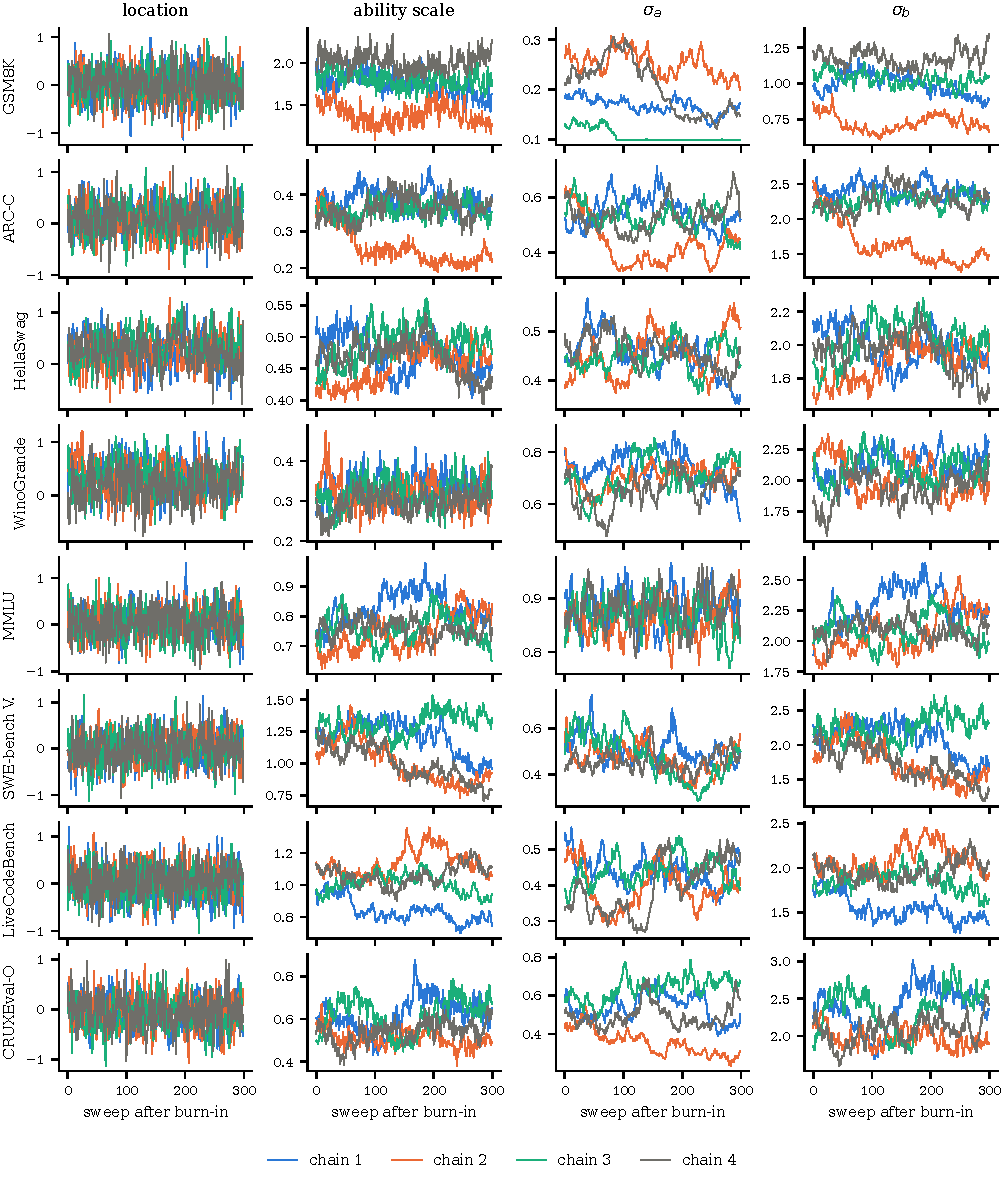
\includegraphics[width=\linewidth]{figures/rf2_traces.pdf}
\caption{Follow-up RF2: traces of the overall location (mean calibrator ability), the ability scale (standard deviation of the calibrators' abilities), $\sigma_a$ and $\sigma_b$ for the first selected panel of each benchmark; four chains (chain 1 starts at EOST-M's estimates), 300 sweeps after a burn-in of 250.}
\label{fig:rf2traces}
\end{figure}}{}

\IfFileExists{figures/rf2d_traces.pdf}{%
\begin{figure}[tbp]
\centering
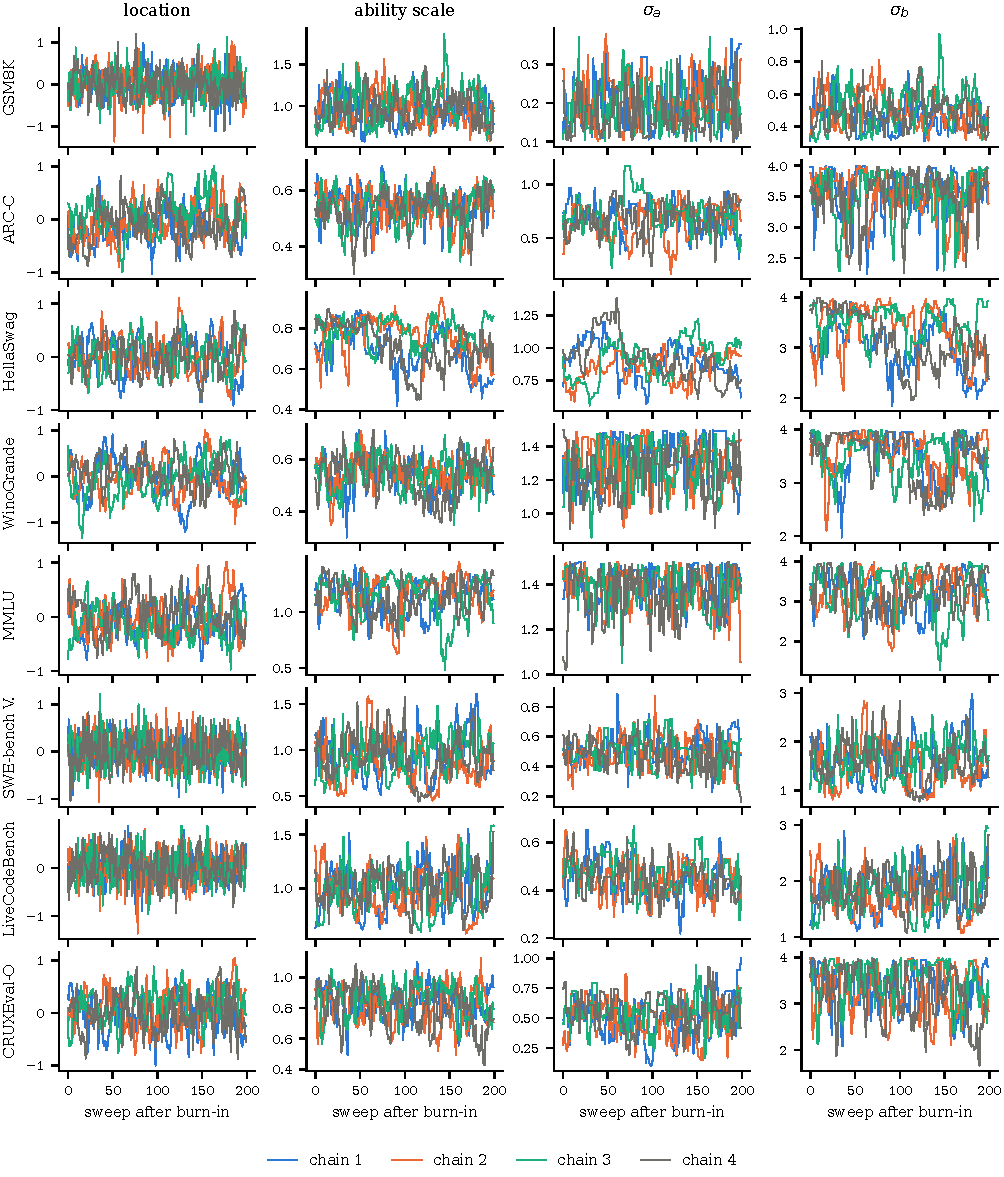
\includegraphics[width=\linewidth]{figures/rf2d_traces.pdf}
\caption{Exploratory follow-up RF2d (exact sampler of the model of Lemma~\ref{lem:exact}, with the hyperparameters, the scale and the location moved with the item parameters summed out): traces of the same quantities and panels as in Figure~\ref{fig:rf2traces}; four chains, 200 sweeps after a burn-in of 150.}
\label{fig:rf2dtraces}
\end{figure}}{}

\RobustMCMCScale

\RobustMCMCExact

\RobustMCMCConclusion

\FloatBarrier
\subsection{Effects across benchmarks (RF3, RF3b)}\label{sec:rf3}
\IfFileExists{tables/meta.tex}{\begin{table}[tbp]
\centering\footnotesize
\caption{Cross-benchmark effect of each study-2 superiority hypothesis (follow-up RF3, secondary; no frozen decision changes): random-effects pooled relative improvement of EOST-M (\%) over the eight benchmarks treated as independent, Hartung--Knapp--Sidik--Jonkman 95\% interval, 95\% prediction interval for a new benchmark, $I^2$ (\%), benchmarks with a positive effect and exact two-sided sign-test $p$; ``sources'': 95\% interval when the five Open LLM Leaderboard benchmarks, which share their 395 systems, count as one source (RF3b; four sources, 3 degrees of freedom); frozen decision. $^\ast$Recalibrated EOST-M interval.}
\label{tab:meta}
\setlength{\tabcolsep}{2.5pt}
\begin{tabular}{@{}lrccccccl@{}}
\toprule
EOST-M versus & pooled & 95\% CI & 95\% PI & $I^2$ & pos. & sign $p$ & sources & frozen \\
\midrule
R2 plug-in 2PL, log loss & $+6.0$ & [4.7, 7.2] & [4.3, 7.6] & 7 & 8/8 & 0.008 & [5.7, 7.6] & yes \\
R3 Naive, score IAE & $+50.5$ & [37.0, 64.0] & [24.2, 76.8] & 87 & 8/8 & 0.008 & [43.5, 57.5] & yes \\
R4 plug-in 2PL, $|\mathrm{cov}-0.9|$ & $+41.9$ & [35.3, 48.6] & [33.6, 50.3] & 6 & 8/8 & 0.008 & [34.0, 45.5] & yes \\
C1 Rasch-type plug-in, log loss & $+2.6$ & [1.2, 4.1] & [$-$0.2, 5.5] & 71 & 7/8 & 0.070 & [$-$0.4, 5.0] & yes \\
C2 Rasch-type marginal, log loss & $+2.0$ & [0.8, 3.2] & [$-$0.6, 4.7] & 75 & 8/8 & 0.008 & [1.4, 2.8] & no \\
C4 Random:mg, score IAE & $+23.4$ & [9.8, 37.1] & [$-$16.5, 63.3] & 88 & 8/8 & 0.008 & [$-$5.0, 52.6] & no \\
C5b raw interval$^\ast$, interval score & $-5.8$ & [$-$19.9, 8.3] & [$-$42.7, 31.0] & 82 & 4/8 & 1.000 & [$-$16.1, 10.0] & no \\
C6 Naive (Wilson)$^\ast$, interval score & $+29.8$ & [9.9, 49.7] & [$-$17.9, 77.5] & 91 & 7/8 & 0.070 & [18.7, 51.1] & yes \\
C7 ATLAS-style, score IAE & $+27.1$ & [11.2, 43.0] & [$-$20.0, 74.2] & 93 & 8/8 & 0.008 & [$-$1.1, 42.4] & no \\
C8 tinyBenchmarks, error @50 & $+34.5$ & [20.0, 49.0] & [$-$3.9, 72.9] & 80 & 8/8 & 0.008 & [$-$1.8, 76.7] & no \\
C9 MINCE, error @50 & $+41.9$ & [26.0, 57.8] & [1.2, 82.6] & 85 & 8/8 & 0.008 & [34.1, 49.3] & yes \\
\bottomrule
\end{tabular}
\end{table}
}{}

\RobustMetaText
